
\noindent\textbf{4. (CRLS 23.1-2)} Prove ou desprove a seguinte afirmação: Dado um grafo $G$ com pesos nas arestas, um conjunto de arestas $A$ de $G$, e um corte que respeita $A$, toda aresta que cruza o corte e que é segura para $A$ tem peso mínimo dentre todas as arestas desse corte.\\[6pt]
\textbf{Resposta:} Seja $A$ formado pelas arestas $\{(t, s), (t, u)\}$, como pode ser visto na figura \ref{fig:8.4-1}.

\begin{center}
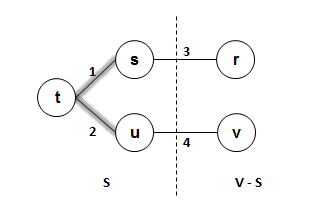
\includegraphics[width=0.45\textwidth]{q8-04.png}
\captionof{figure}{Exemplo de grafo com uma única MST contendo aresta de não peso mínimo no corte.}
\label{fig:8.4-1}
\end{center}

O corte $(S, V - S)$ respeita $A$. $(u, v)$ é uma aresta que atravessa o corte $(S, V - S)$ e é segura para $A$, ou seja, $A \cup \{(u, v)\} \subseteq T$, porém, não é de custo mínimo (\textit{light edge}).